\subsection{Cómo revisar los métodos de pago}
Para revisar los medios de pago, se debe ingresar a la pestaña de “Mi perfil”, donde se debe dar clic en “Mis Métodos”.

\begin{figure}[H]
    \centering
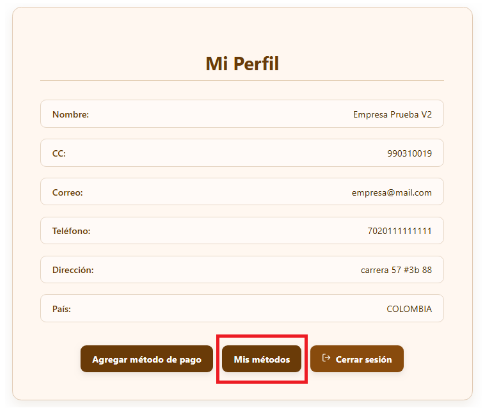
\includegraphics[width=0.6\linewidth]{casosuso/perfil-mismetodos.png}
\caption{Perfil, botón mis métodos.}
\label{fig:perfil-mismetodos}
\end{figure}

Luego, en la interfaz, se verán los métodos de pago registrados:

\begin{figure}[H]
    \centering
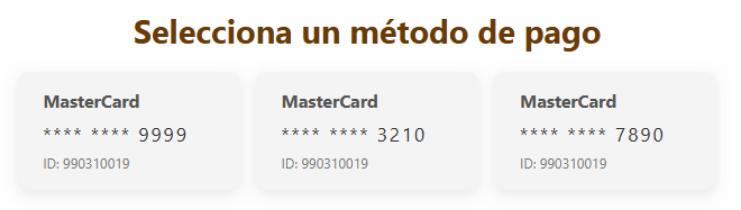
\includegraphics[width=0.8\linewidth]{casosuso/mismetodos.png}
\caption{Métodos registrados por el usuario.}
\label{fig:mismetodos}
\end{figure}

\subsection{Cómo transferir un dominio}
Para esto se debe ingresar a “Mis dominios”, de la siguiente forma:

\begin{figure}[H]
    \centering

\includegraphics[width=0.8\linewidth]{casosuso/navbar-misdominios.png}
\caption{Barra de navegación, Mis dominios.}
\label{fig:navbar-misdominios}
\end{figure}

Luego del listado de dominios del usuario como se ve en la figura \ref{fig:domino-usuario} se debe seleccionar el dominio que desea transferir.\\\\
A, continuación  se debe ingresar el correo electrónico, de la cuenta a la que se desea transferir, de la siguiente manera:

\begin{figure}[H]
    \centering
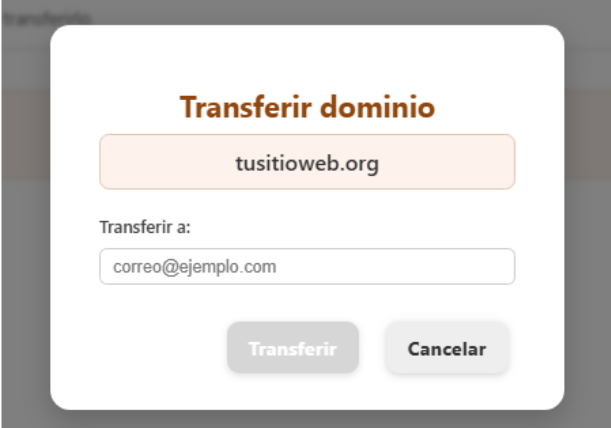
\includegraphics[width=0.6\linewidth]{casosuso/dominios-transferir.png}
\caption{Transferir dominio.}
\label{fig:dominios-transferir}
\end{figure}

Finalmente, se verá el siguiente mensaje de confirmación
\begin{figure}[H]
    \centering
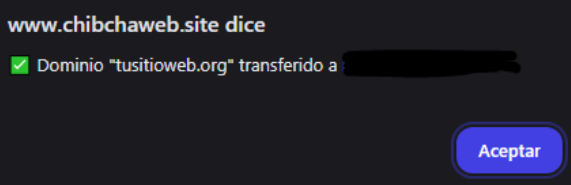
\includegraphics[width=0.6\linewidth]{casosuso/dominios-aviso.png}
\caption{Transferir dominio, notificación.}
\label{fig:dominios-aviso}
\end{figure}
